\documentclass[12pt]{article}
\usepackage{graphicx}
\usepackage{sectsty}
\usepackage{titlesec}
\usepackage{listings}
\usepackage{xcolor}
\usepackage{amsmath, nccmath}
\usepackage{geometry}

\colorlet{codecolor}{black!30}
\newcommand{\codebox}[1]{%
	\colorbox{codecolor}{\ttfamily \detokenize{#1}}%
}

\geometry{
	a4paper,
	total={170mm,257mm},
	left=20mm,
	top=20mm,
}

\definecolor{codegreen}{rgb}{0,0.6,0}
\definecolor{codegray}{rgb}{0.5,0.5,0.5}
\definecolor{codepurple}{rgb}{0.58,0,0.82}
\definecolor{backcolour}{rgb}{0.95,0.95,0.92}

\lstdefinestyle{mystyle}{
	backgroundcolor=\color{backcolour},   
	commentstyle=\color{codegreen},
	keywordstyle=\color{magenta},
	numberstyle=\tiny\color{codegray},
	stringstyle=\color{codepurple},
	basicstyle=\ttfamily\footnotesize,
	breakatwhitespace=false,         
	breaklines=true,                 
	captionpos=b,                    
	keepspaces=true,                 
	numbers=left,                    
	numbersep=5pt,                  
	showspaces=false,                
	showstringspaces=false,
	showtabs=false,                  
	tabsize=2
}

\lstset{style=mystyle}

%%%%%%%%%%%%%%%%%%%%%%%%%%%%%%%%%%%%%%%%%%%%%%%%%%%%%%%%%%%%%


\titleformat*{\section}{\huge\bfseries\sffamily}
\sectionfont{\fontsize{14}{0}\selectfont}

\titleformat{\section}
{\sffamily\Large\bfseries}{\thesection}{1em}{}[{\titlerule[1.2pt]}]


\title{\huge\textbf{Data Mining on IPL Dataset}}
\author{\large\textbf{GROUP ID - 26}\\ \large\textbf{Mid Semester Report}}
\date{\LARGE\textbf{18 October 2020}}


\begin{document}
\maketitle
\vspace{20pt}
\begin{figure}[h]
\centering

\includegraphics[scale=1]{iitk2.jpg}
\end{figure}

\vspace{20pt}

{\Large{\begin{center}
	\textbf{GROUP MEMBERS:}
	\vspace*{7pt}
	
	\begin{tabular}{c c c}
		Aditya Raghuwanshi & 170052 & adityarg@iitk.ac.in \\ 
		Ritesh Naik & 170579 & riteshn@iitk.ac.in \\ 
		Shashi Kumar & 160646 & shashik@iitk.ac.in \\
	\end{tabular}
\end{center}}}
\newpage
%%%%%%%%%%%%%%%%%%%%%%%%%%%%%%%%%%%%%%%%%%%%%%%%%%%%%%%%%%%%%%%%%%%%%

\section*{Abstract}
The Indian Premier League (IPL) is a professional Twenty20 cricket league in India usually contested between March and May of every year by eight teams representing eight different cities or states in India. IPL is very popular among cricket fans in India and is getting more liked by the hihg intensity \& competitive nature of the game. Many official \& unofficial sources has been collecting data from IPL matches from 2008. Like other domains, we can use this data to analyse weaknesses/strengths of the players and teams, or an overall performance of the campaign. This type of analysis can be useful for teams and also for prediciting viewership. This report includes some of the basic analysis.


\section*{Introduction \& Motivation}



\section*{Aims of the project}
\begin{enumerate}
\item To visualize different stats of players and teams throughout the seasons.
\item Classify players according to their performance into specific groups.
\item Find the scores of each player(or rank them) according to their performance in IPL.
\item Create a best 11 team for IPL using previous scores and other constraints.
\item To study data to find the relation of unconventional factors on each team results like Home ground - Away ground, Toss Winning - Toss Losing, etc.
\item To predict expected number of boundaries (fours \& sixes) and targets using previous season stats.
\end{enumerate}


%%%%%%%%%%%%%%%%%%%%%%%%%%%%%%%%%%%%%%%%%%%%%%%%%%%%%%%%%%%%%%%%%%%%%

\section*{Dataset Needed}
\paragraph{}
We have identified two data sources that is suites our need:

	\subsection*{1. Official IPL Dataset}
	
	It contains following stats:\\
	\begingroup
	\setlength{\tabcolsep}{15pt} % Default value: 6pt
	\renewcommand{\arraystretch}{1.3} % Default value: 1
	\begin{tabular}{ l l}
		\textbullet Most Runs & \textbullet Most Maidens \\
		\textbullet Most Runs (Over) & \textbullet Most Dot Balls \\
		\textbullet Most Fours & \textbullet Most Dot Balls (Innings) \\
		\textbullet Most Fours (Innings) & \textbullet Best Bowling Average \\
		\textbullet Most Sixes & \textbullet Best Bowling Economy \\
		\textbullet Most Sixes (Innings) & \textbullet Best Bowling Economy (Innings) \\
		\textbullet Most Fifties & \textbullet Best Bowling Strike Rate \\
		\textbullet Most Centuries & \textbullet Best Bowling Strike Rate (Innings) \\
		\textbullet Fastest Fifties & \textbullet Best Bowling Innings \\
		\textbullet Fastest Centuries & \textbullet Most Run Conceded (Innings) \\
		\textbullet Highest Scores & \textbullet Fastest Balls \\
		\textbullet Highest Scores (Innings) & \textbullet Most Hat Tricks \\
		\textbullet Best Batting Strike Rate & \textbullet Most Four Wickets \\
		\textbullet Best Batting Average & \textbullet Player Points \\
		\textbullet Biggest Sixes & \textbullet Team Ranking \\
		\textbullet Most Wickets &  \\
	\end{tabular}
	\newline\newline\newline
	Some points about the data:
	\begin{enumerate}
		\itemsep -0.2em 
		\item It contains stats / data of all seasons from 2008 to 2019.
		\item It does NOT contain match wise data and player wise data.
		\item As it does not contain match wise data, extracting IPL 2020 data now is not meaningful
	\end{enumerate}
	
	\subsection*{2. Kaggle IPL Dataset}
	
	It contains following files:\\
	\begingroup
	\setlength{\tabcolsep}{6pt} % Default value: 6pt
	\renewcommand{\arraystretch}{1.3} % Default value: 1
	\begin{tabular}{ l l}
		\textbullet \textbf{deliveries.csv}: & Statistics of each ball of each match\\
		\textbullet \textbf{matches.csv}: & Overall statistics of each match\\
		\textbullet \textbf{teamwise\_home\_and\_away.csv}: & Home and Away win percentages of each team\\
		\textbullet \textbf{Players.xlsx}: & Contains details about player name, date of birth,\\ & country of origin, batting and bowling preference\\
		\textbullet \textbf{teams.csv}: & Names of each match\\
	\end{tabular}
	\newline\newline\newline
	Some points about the data:
	\begin{enumerate}
		\itemsep -0.2em 
		\item It contains stats / data of all seasons from 2008 to 2019.
	\end{enumerate}


\section*{Sources of Dataset}
	\subsection*{1. Official IPL Dataset}
	We have extracted dataset from IPL official website using a PyInquirer Application built from python. We can choose feature(s) and year(s) to get required data.
	
	\begin{itemize}
		\itemsep 0em
		\item Select years from 2008 to 2019 or "all-time" records and select some of or all of the given stats.
		\item We call the function get\_year\_stats() in our main() function. This function then obtains HTML from the url, creates its soup object and passes it to get\_years() and get\_stats() methods. URL has following format:
		\item[] \textbf{https://www.iplt20.com/stats/ + $<$year/$>$ + $<$stats name$>$}
		\item The stats have two variables stats\_url, stats\_title. The former store page name of the stats page and the latter stores the title that will be displayed to the user.
		\item \textbf{get\_years(soup)}, extracts years data from the website. \textbf{re.compile}, creates a regex to find tags having ‘sub-menu’ as a substring in its class name. textbf{soup.find\_all}, finds all the ‘a’ tags with the specified class name. \textbf{year.get\_text()}, creates a list comprehension by applying get\_text() function on all the elements of the result of the find\_all() method.
		
		\begin{lstlisting}[language=Python]
			soup = BeautifulSoup(page.content, 'html.parser')
			years= year.get_text() for year in soup.find_all('a',class_=re.compile(r'sub-menu*'))\end{lstlisting}
	
		\item We replace ‘All Time Records’ with ‘all-time’. Former being display name and latter being the part of the URL.
		\begin{lstlisting}[language=Python]
			years[-1] = 'all-time'\end{lstlisting}
		\item Similarly, we will extract the stats name and stats page name in \textbf{get\_stats(soup)} function.
		\begin{lstlisting}[language=Python]
			stats = soup.find_all('a', class_=re.compile(r'side*'))\end{lstlisting}
		
		\item We will use the \textbf{\textit{years}} list to create a list of dictionary with \textbf{\textit{name}} as key and \textbf{\textit{year}} as value.
		
		\item We will use the \textbf{\textit{stats\_title}} list as name to be displayed to the user and \textbf{\textit{stats\_url}} as its value, which will be returned to the program when a user selects a particular stats.
		\begin{verbatim}
			For eg, name: Most Runs and respective value: most-runs.
			Value is the name of the page in URL and the name is the title of the page.
		\end{verbatim}
		
		\item The following code prepares a PyInquirer query and stores their response in answers variable. Here we are using a while loop to handle no response from the user, TypeError to handle CTRL + C and EOFError to handle CTRL + D.
		
		\begin{lstlisting}[language=Python]
def user_input(years_q, stats_q, kanpeki):
    answers = {'years': '', 'stats': ''}
	try:
		while len(answers.get('years')) == 0 or len(answers.get('stats')) == 0:
			questions = [
			{
				'type': 'checkbox',
				'message': 'Select type',
				'name': 'years',
				'choices': years_q,
			}, {
				'type': 'checkbox',
				'message': 'Select statistics',
				'name': 'stats',
				'choices': stats_q,
			}
			]
			answers = prompt(questions)
		temp = {'years': ''}
		if answers['years'][0]=='By Season Stats':
			while len(temp.get('years')) == 0:
				questions = [
				{
					'type': 'checkbox',
					'message': 'Select years',
					'name': 'years',
					'choices': kanpeki,
				}
			]
			temp=prompt(questions)
			answers['years']=temp['years']
	except TypeError:
		error_msg()
	except EOFError:
		exit_application()
	return answers['years'], answers['stats']
		\end{lstlisting}
	
	\item We have obtained year values, stats values (page name and page title) and created a query to obtain user response and store it in a variable called \textbf{\textit{answers}}.
	
	\item To extract player’s data, we define a function called \textbf{\textit{scrap\_data(years, stats)}} that will iterate over all the selected value of years and stats page names.
	
	\begin{lstlisting}[language=Python]
def scrap_data(years, stats):
	base = 'https://www.iplt20.com/stats/'
	base_file_name = 'Result'
	for year in years:
		for stat in stats:
			if stat == 'team-ranking':
				url = base + year
				data, columns = get_page(url, True)
				data_set_name = 'Team-Ranking-' + year
			else:
				url = base + year + '/' + stat
				print(url)
				data, columns = get_page(url, False)
				data_set_name = str.title(stat) + '-' + year
			if len(data) == 0:
				print(data_set_name + ' :' + 'Data not Available')
			else:
				save_data(data, columns, data_set_name, base_file_name)
	\end{lstlisting}

	\item All the pages of the first type have the same HTML layout and the same goes for the second type. As stated in the first case we don’t need any page name and in the second case, the stats name is concatenated to our base URL.
	\item We then define a function called \textbf{\textit{get\_page(url, team)}} that will do a preliminary check and create a soup object of the page. The team argument is a boolean value set to True for the first type of page and False for the second type.
	
	We call \textbf{\textit{find\_col(soup, team)}} function in \textbf{\textit{get\_page(url, team)}} which will return the header values of all the columns present in the table on the webpage.
	\begin{lstlisting}[language=Python]
		def get_page(url, team):
			try:
				page = requests.get(url)
				if page.status_code == 200:
					soup = BeautifulSoup(page.content, 'html.parser')
					data, columns = find_col(soup, team)
					return data, columns
				else:
					print('Website Unreachable')
					return
			except requests.exceptions.ConnectionError:
				print('Please check network connection')
				return
	\end{lstlisting}
	\item The \textbf{\textit{find\_col(soup, team)}} will find the column headers, and \textbf{\textit{get\_team\_data(soup, columns)}} and \textbf{\textit{get\_player\_data(soup, columns)}} will scrape the first and second type of data.
	
	\begin{lstlisting}[language=Python]
def find_col(soup, team):
	try:
		if team:
			columns = list(filter(None, soup.find('tr', class_='standings-table__header').get_text().split('\n')))
			return get_team_data(soup, columns)
		else:
			columns = re.sub(r'\n[\s]*', '\n',soup.find('tr', class_=re.compile(r'top-players__header*')).get_text()).strip().split('\n')
			return get_player_data(soup, columns)
	except AttributeError:
		return [], []
	
	
def get_team_data(soup, columns):
	data = []
	for i in soup.find_all('td'):
		data.append(re.sub(r'\n[\s]*', " ", i.get_text().strip()))
	data = np.array(data).reshape(len(data) // len(columns), len(columns) + 1)
	data = np.delete(data, 0, axis=1)
	return data, columns
	
	
def get_player_data(soup, columns):
	data = []
	for i in soup.find_all('td', class_=re.compile(r'top-players*')):
		data.append(re.sub(r'\n[\s]*', " ", i.get_text().strip()))
	data = np.array(data).reshape(len(data) // len(columns), len(columns))
	return data, columns
	\end{lstlisting}
	
	\item Line \#4 command finds all the ‘TR’ tags with the specified class name, extracts text from it and then splits it to form a list. At last, remove the blank value to get all the column headers.
	
	\item[] Line \#7 finds ‘TR’ tags with class that has ‘top\_players\_header’ present in the class name, gets text from it substitute all the newline and space characters with just new line characters and then remove the blank space. At last splits it using ‘\textbackslash n’ as a delimiter to form a list.
	
	\item[] Line \#17 extracts all the ‘TD’ tags and formats the values to get all the team data.
	
	\item[] Line \#26 extracts player data with tag name ‘TD’ and class having ‘top-players’ substring. After which formats it to form a list called data.
	
	\item Line \#26 of the function \textbf{\ textit{get\_player\_data(soup, columns)}} we convert the data list to a data numpy array and also reshape it from a 1D array to a 2D array. The number of columns is specified by the length of the column list and the number of rows by integer division of length of data list by the length of the columns list. The same goes for the third last line of \textbf{\textit{get\_team\_data(soup, columns)}}.
	
	\item We now extracted the data in a numpy 2d array called \textbf{\textit{data}} and column headers in a list called \textbf{\textit{columns}}.
	
	\item We will create a \textbf{\textit{save\_data(data, columns, data\_set\_name, file\_name)}} function which will create a dataframe from the data and a file path based on the data in the dataframe. After which it will save dataframe in the form of a CSV and notify the user.
	\begin{lstlisting}[language=Python]
def save_data(data, columns, data_set_name, file_name):
	df = pd.DataFrame(data, columns=columns)
	file_path = './' + file_name + '-' + data_set_name + '.csv'
	df.to_csv(file_path, index=False)
	print(data_set_name + ' saved as: ' + os.path.dirname(os.path.abspath(__file__)) + '/' + data_set_name + '.csv')
	\end{lstlisting}
	
	\item The \textbf{\textit{main()}} function will call \textbf{\textit{get\_year\_stats()}} to get year values, stats page names and titles.
	After which we will call \textbf{\textit{prepare\_question(years, stats\_title, stats\_url)}} to prepare the query for the user. We will get user’s input from \textbf{\textit{user\_input(years\_q, stats\_q)}} function and then get scrapping by calling \textbf{\textit{scrap\_data(years, stats)}} function.
	\begin{lstlisting}[language=Python]
def main():
	years, stats_url, stats_title = get_year_stats()
	years_q, stats_q = prepare_question(years, stats_title, stats_url)
	years, stats = user_input(years_q, stats_q)
	print('Collecting and saving data.')
	scrap_data(years, stats)
	\end{lstlisting}
	
	\item Screenshots of the application
	\begin{figure}[h]
		\centering
		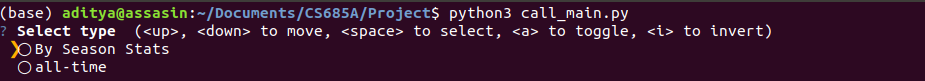
\includegraphics[scale=0.5]{app1.png}
	\end{figure}
	\begin{figure}[h]
		\centering
		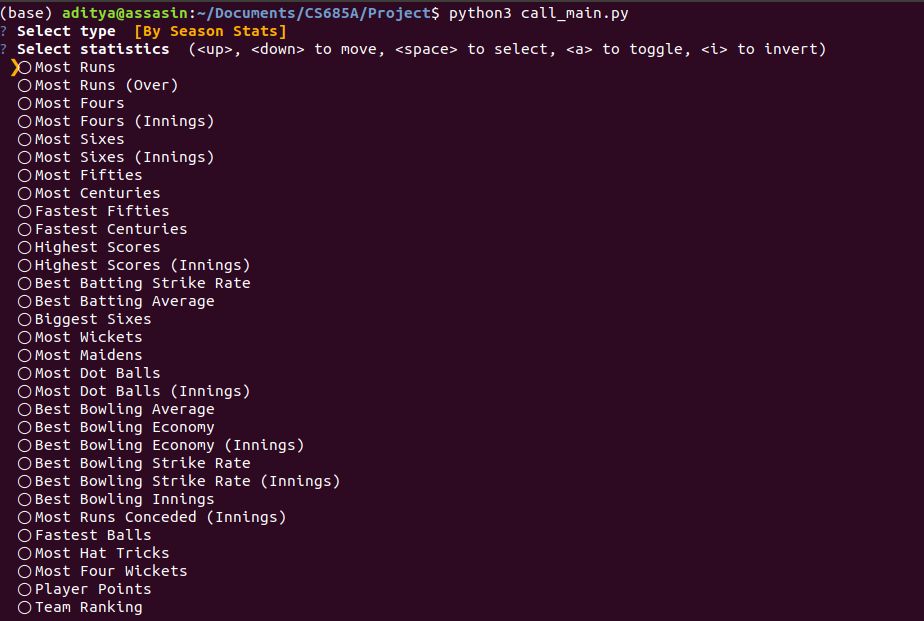
\includegraphics[scale=0.5]{app2.png}
	\end{figure}
	\begin{figure}[h]
		\centering
		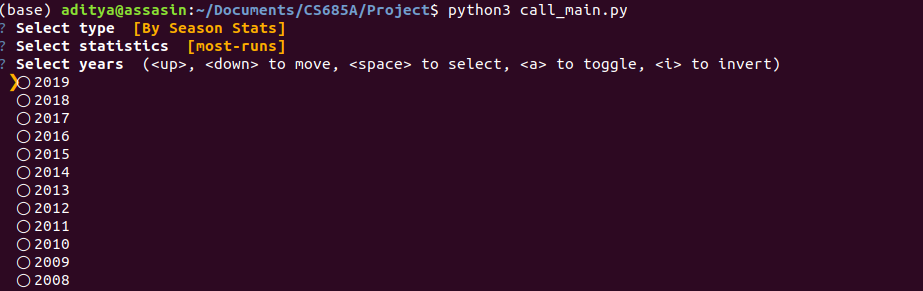
\includegraphics[scale=0.5]{app3.png}
	\end{figure}
	
	\end{itemize}


\newpage
	\subsection*{2. Kaggle IPL Dataset}
	All the files "deliveries.csv", "matches.csv", "teamwise\_home\_and\_away.csv", "Players.csv" and "teams.csv" are directly available from the Kaggle website to download.



%%%%%%%%%%%%%%%%%%%%%%%%%%%%%%%%%%%%%%%%%%%%%%%%%%%%%%%%%%%%%%%%%%%%%%%%%


\section*{Methodology to meet the Aims}
Each point will corresponds to previous points in the Aims .

\begin{enumerate}
	\itemsep -0.1em 
	\item  For visualization and data presentation , we are going to use different libraries of python and different types of graphs . The main objective is to clean , modify and structure the data accordingly such that it will be easier for us to complete future objectives .
	\item We are going to use clustering algorithm to classify the players given their cricket statistics. For example , the given figure is obtained after a clustering algorithm. Similary, we can apply this method in player's data and group them into different categories such that pink might refer to opening batsman, green might refer to middle order and blue might refer to hitter batsman.
	
	\begin{figure}[h]
		\centering
		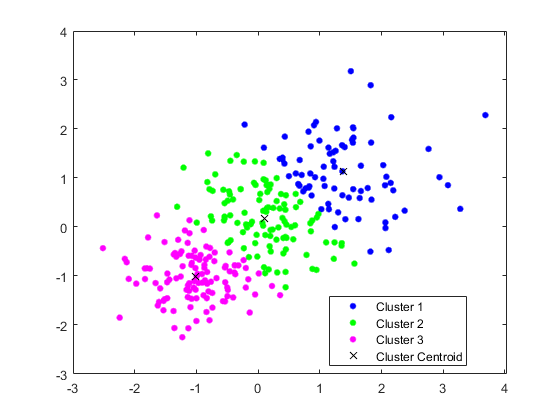
\includegraphics[scale=0.45]{cluster.png}
	\end{figure}
	
	\item Score of a player will measure the ability or contribution of a player to the team .We are going to use the different datas of the player's performance in the IPL to find his score .Ranking algorithm can be used to rank the players in the specific criteria . Points of a player is also available in the IPL official website , which we can use to compare our scores with those points.\\
	\textbf{RANKING ALGORITHM:}\\
	$\textbf{Opening Batsman Score} =  \dfrac{\mfrac{total runs}{total matches}}{30} + \mfrac{Strike Rate}{100}$\\
	$\textbf{Middle Order Batsman Score} =  \mfrac{Number Of Sixes}{Max Number Of Sixes} + \mfrac{Strike Rate}{100}$\\
	$\textbf{Bowler Scores} =  \mfrac{Wickets}{Max Wickets} + \mfrac{7}{Economy}$\\
	
	\item To find the best 11 players of the tournament, I have used results from clustering and ranking algortihm discussed above. From each clusters, I have taken best players according to their scores. I have taken 4 from upper batsmen, 3 from middle order, and 4 from bowlers. We can also manually take indian players for best indian team. We can alter the number of upper batsman, middle order and bowlers as required.
	
	\item Our kaggle dataset contains \codebox{teamwise_home_and_away.csv} file. We are performing a simple operation. First, scale total number of matches to 100, because all the teams have played different number of matches. Then, we will find the ratio of "home wins" to "away wins" for each team. If the ratio$>>$1 for the team, then team performs better on home ground, else if the ratio$<<$1, then team performs better on away ground.
	
	Our kaggle dataset contains \codebox{teams.csv} file. Get the total number of tosses won and tosses lost. Get the total number of matches won when the team loose the toss and also when won the toss. Normalize everything to 100 and take ratio. Ratio is defined as percent of matches won when toss is won by percent of matches won when toss is lost.
	
	\item From the official IPL dataset, when can fetch top 100 players with most number of 4s(boundaries). Total number of 4s was not available in any data. So, we assumed that total number of 4s in a season is equivalent to total number of most 4s by 100 players. We calculated this data for each season from 2008 to 2019.
	
	We can do similar operation to find total and average number of sixes scored across each season.
	
\end{enumerate}




\newpage
\section*{Results}

\subsection*{CLUSTERING}


\subsubsection*{Opening Batsman}
\hrule
\begin{tabular}{c | c | c | c}
	KL Rahul & Quinton de Kock & Shikhar Dhawan & Suryakumar Yadav \\
	David Warner & Ishan Kishan & AB de Villiers & Faf du Plessis \\
	Mayank Agarwal & Devdutt Padikkal & Eoin Morgan & Shreyas Iyer \\
	Manish Pandey & Ben Stokes & Shubman Gill & Nitish Rana \\
	Rohit Sharma & Jonny Bairstow & Rishabh Pant & Jos Buttler \\
	Shane Watson & Ambati Rayudu & Chris Gayle & Steve Smith \\
	Kane Williamson & Aaron Finch & Wriddhiman Saha & Ruturaj Gaikwad \\
\end{tabular}


\subsubsection*{Middle Order Batsman}
\hrule
\begin{tabular}{c | c | c | c}
	Rahul Tewatia & Marcus Stoinis & Sam Curran & Ravindra Jadeja \\
	Kieron Pollard & Sanju Samson & Nicholas Pooran & Sunil Narine \\
	Hardik Pandya & Andre Russell & Prithvi Shaw & MS Dhoni \\
	Virat Kohli & Rahul Tripathi & Shimron Hetmyer & Dinesh Karthik \\
	Glenn Maxwell & Robin Uthappa & Shivam Dube & Vijay Shankar \\
	Abdul Samad & Tom Curran & Priyam Garg & Ajinkya Rahane \\
	Abhishek Sharma & Mandeep Singh & Deepak Hooda & Saurabh Tiwary \\
	Gurkeerat Mann Singh & Riyan Parag & Krishnappa Gowtham & Josh Philippe \\
	Kedar Jadhav & Sarfaraz Khan & Mahipal Lomror & Yashasvi Jaiswal \\
	Narayan Jagadeesan & Murali Vijay & Mohammad Nabi & Simran Singh \\
	Tom Banton & Rinku Singh \\
\end{tabular}


\subsubsection*{Bowlers}
\hrule
\begin{tabular}{c | c | c | c}
	Jofra Archer & Kagiso Rabada & Jasprit Bumrah & Rashid Khan\\
	Trent Boult & Anrich Nortje & Pat Cummins & Mohammad Shami \\
	T Natarajan & Yuzvendra Chahal & Axar Patel & Varun Chakravarthy \\
	Washington Sundar & Ravi Bishnoi & Krunal Pandya & Sandeep Sharma \\
	Deepak Chahar & Rahul Chahar & Ravichandran Ashwin & Chris Morris \\
	Navdeep Saini & Shreyas Gopal & Mohammed Siraj & Jason Holder \\
	James Pattinson & Kartik Tyagi & Murugan Ashwin & Chris Jordan \\
	Shardul Thakur & Shivam Mavi & Nathan Coulter-Nile & Arshdeep Singh \\
	Khaleel Ahmed &  Isuru Udana & Lockie Ferguson & Sheldon Cottrell \\
	Kamlesh Nagarkoti & Lungi Ngidi & Dwayne Bravo & Piyush Chawla \\
	Shahbaz Nadeem & Prasidh Krishna & Jaydev Unadkat & Tushar Deshpande\\
	Bhuvneshwar Kumar & Karn Sharma & Ankit Rajpoot & Harshal Patel \\
	Jimmy Neesham & Josh Hazlewood & Amit Mishra & Daniel Sams \\
	Adam Zampa & Imran Tahir & Dale Steyn & Kuldeep Yadav \\
	Mitchell Santner & Varun Aaron & Shahbaz Ahmed & Jayant Yadav \\
	Moeen Ali & Pravin Dubey & Umesh Yadav & Siddarth Kaul \\
	Mujeeb Ur Rahman & Andrew Tye & Mohit Sharma & Alex Carey \\
	Basil Thampi & Sandeep Warrier & Karun Nair & Avesh Khan \\
	Harpreet Brar & Chris Green & Dhawal Kulkarni & Monu Kumar \\
	Ishant Sharma & Nikhil Naik & Shreevats Goswami & Mitchell Marsh \\
	David Miller & & & \\
\end{tabular}


\subsection*{RANKING}

\begin{minipage}{240pt}
	\subsection*{Opening Batsman}
	\hrule
	\begin{tabular}{c | c}
		\textbf{Players} & \textbf{Scores}\\
		KL Rahul & 2.888638095238095 \\
		Mayank Agarwal & 2.849348484848485 \\
		Ishan Kishan & 2.6861714285714284 \\
		Shikhar Dhawan & 2.6590647058823524 \\
		AB de Villiers & 2.596288888888889 \\
		Faf du Plessis & 2.5587820512820514 \\
		Nicholas Pooran & 2.5375761904761904 \\
		David Warner & 2.4880666666666666 \\
		Sanju Samson & 2.4817571428571426 \\
		Kieron Pollard & 2.4725333333333332 \\
	\end{tabular}
\end{minipage}
\begin{minipage}{240pt}
	\subsection*{Middle Order Batsman}
	\hrule
	\begin{tabular}{c | c}
		\textbf{Players} & \textbf{Scores}\\
		Kieron Pollard & 2.647533333333333 \\
		Hardik Pandya & 2.623133333333333 \\
		Nicholas Pooran & 2.5304333333333333 \\
		Ishan Kishan & 2.4576000000000002 \\
		Sanju Samson & 2.4555666666666665 \\
		AB de Villiers & 2.3540666666666668 \\
		Eoin Morgan & 2.1841 \\
		Quinton de Kock & 2.138333333333333 \\
		Chris Gayle & 2.1380666666666666 \\
		Jofra Archer & 2.1269333333333336 \\
	\end{tabular}\\
\end{minipage}

\begin{minipage}{240pt}
	\subsection*{Bowlers}
	\hrule
	\begin{tabular}{c | c}
		\textbf{Players} & \textbf{Scores}\\
		Rashid Khan & 1.9702048417132216 \\
		Jasprit Bumrah & 1.940118870728083 \\
		Kagiso Rabada & 1.839328537170264 \\
		Jofra Archer & 1.7353689567430024 \\
		Trent Boult & 1.7116269343370976 \\
		Yuzvendra Chahal & 1.6887005649717515 \\
		Varun Chakravarthy & 1.5900584795321637 \\
		Anrich Nortje & 1.5676599125943582 \\
		Mohammad Shami & 1.483469467133411 \\
		Washington Sundar & 1.4411633109619686 \\
	\end{tabular}=\\
\end{minipage}


\subsection*{Best 11 Players}

\begin{tabular}{c | c}
	\textbf{Players} & \textbf{Scores}\\
	KL Rahul & 2.888638095238095\\
	Mayank Agarwal & 2.849348484848485\\
	Ishan Kishan & 2.6861714285714284\\
	Shikhar Dhawan & 2.6590647058823524\\
\end{tabular} \hspace*{50pt} \textbf{Opening Batsman with their score}\\
\\\\
\begin{tabular}{c | c}
	\textbf{Players} & \textbf{Scores}\\
	Kieron Pollard & 2.647533333333333\\
	Hardik Pandya & 2.623133333333333\\
	Nicholas Pooran & 2.5304333333333333\\
\end{tabular} \hspace*{30pt} \textbf{Middle Order Batsman with their score}\\
\\\\
\begin{tabular}{c | c}
	\textbf{Players} & \textbf{Scores}\\
	Rashid Khan & 1.9702048417132216\\
	Jasprit Bumrah & 1.940118870728083\\
	Kagiso Rabada & 1.839328537170264\\
	Jofra Archer & 1.7353689567430024\\
\end{tabular} \hspace*{60pt} \textbf{Bowlers with their score}\\


\subsection*{HOME-AWAY MATCHES}
\hrule
\vspace*{15pt}
\textbf{Ratio $\rightarrow LEAST: \leq 0.1 ;;  0.1 < MODERATE \leq 0.4 ;;  0.4 < MOST$}

\textbf{LEAST} effect on home-away games: Rising Pune Supergiant \& Mumbai Indians\\
\textbf{MOST} effect on home-away games : Kochi Tuskers Kerala \& Gujarat Lions have most impact on home-away games\\
Rest have \textbf{MODERATE} effects.

Rising Pune Supergiant, Kochi Tuskers Kerala \& Gujarat Lions have played very few matches relative to other teams, so it is expected that they will move to MODERATE section after several matches.
Only Mumbai Indians show very less effect after playing significant matches.


\begin{figure}
	\centering
	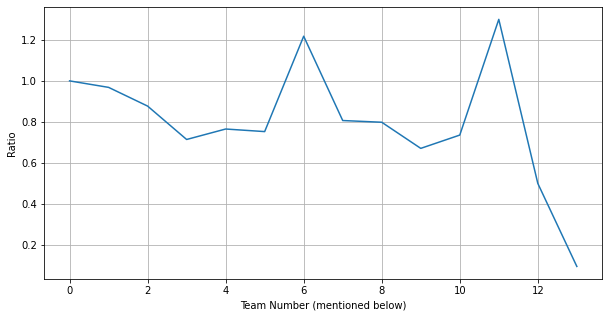
\includegraphics[width=0.7\linewidth]{home_away}
	\caption{Ratio of home-away wins of each team}
	\label{fig:homeaway}
\end{figure}


{\fontsize{10}{12}\selectfont \begin{tabular}{l | l | l | l}
		0:Rising Pune Supergiant & 1:Mumbai Indians & 2:Chennai Super Kings & 3:Delhi Capitals\\
		4:Sunrisers Hyderabad & 5:Rajasthan Royals & 6:Deccan Chargers & 7:Kings XI Punjab\\
		8:R. Challengers Bangalore & 9:Kolkata Knight Riders & 10:Delhi Daredevils & 11:Pune Warriors\\
		& 12:Kochi Tuskers Kerala & 13:Gujarat Lions & \\
\end{tabular}}
\\\\\\
Execpt \textbf{Deccan Chargers} \& \textbf{Pune Warriors}, all other teams have played better in away matches than in home matches.\\

\textbf{Conclusion:} So, on average teams have slight effect of home-away match and most of the teams perform better in away matches.

\subsection*{TOSS WINNING}
\hrule
\vspace*{15pt}
\textbf{Ratio $\rightarrow LEAST: \leq 0.1 ;;  0.1 < MODERATE \leq 0.6 ;;  0.6 < MOST$}
\textbf{LEAST} affected:  ['Rajasthan Royals', 'Mumbai Indians']\\
\textbf{MODERATE} affected:  ['Pune Warriors', 'Kolkata Knight Riders', 'Kochi Tuskers Kerala', 'Chennai Super Kings', 'Rising Pune Supergiants', 'Delhi Daredevils', 'Deccan Chargers', 'Delhi Capitals', 'Sunrisers Hyderabad', 'Royal Challengers Bangalore', 'Kings XI Punjab']\\
\textbf{MOST} affected:  ['Gujarat Lions', 'Rising Pune Supergiant']\\

\begin{figure}
	\centering
	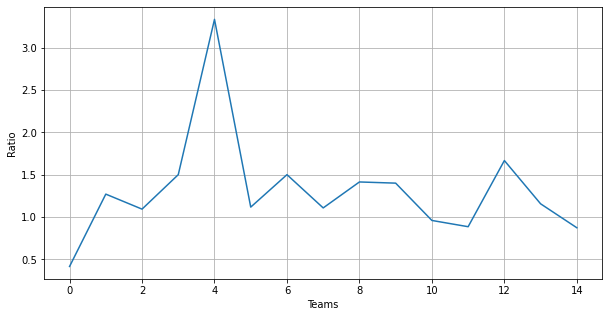
\includegraphics[width=0.7\linewidth]{toss}
	\caption{Ratio of no of toss won \& toss lost for a won match}
	\label{fig:toss}
\end{figure}

Almost all teams won their matches when they won the match toss, except Mumbai Indians, Sunrisers Hydrabad, Pune Warriors, Kings XI Punjab. Out of which Mumbai Indians have LEAST affect and Sunrisers Hydrabad, Pune Warriors, Kings XI Punjab have MODERATE affect.\\\\
\textbf{Conclusion:} Therefore, on average teams win their match when they win the toss

\subsection*{NUMBER OF FOURS (BOUNDARIES)}
\hrule
\vspace*{15pt}

We have tried to find total number of 4s \& average number of 4s. We have used \codebox{moving average} method to model the trend followed throughout the 11 seasons.

{\centering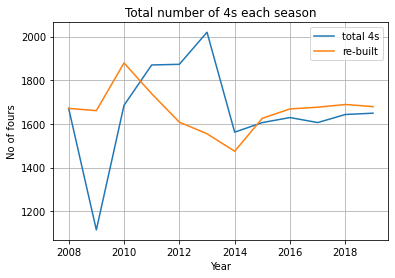
\includegraphics[width=0.5\linewidth]{foursT}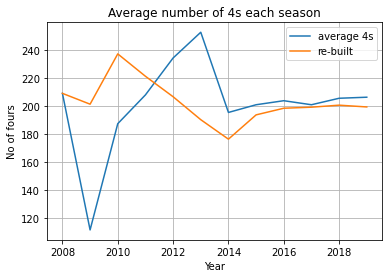
\includegraphics[width=0.5\linewidth]{foursA}}

\textbf{Predicition:} Total number of 4s = 1646\\
\hspace*{75pt} Average number of 4s = 205

\subsection*{NUMBER OF SIXES (BOUNDARIES)}
\hrule
\vspace*{15pt}

From the official IPL dataset, when can fetch top 100 players with most number of sixes(boundaries). Total number of sixes was not available in any data. So, we assumed that total number of sixes in a season is equivalent to total number of most sixes by 100 players. We calculated this data for each season from 2008 to 2019.

We have tried to find total number of sixes \& average number of sixes. We have used \codebox{moving average method} to model the trend followed throughout the 11 seasons.

{\centering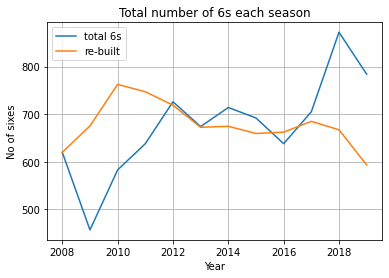
\includegraphics[width=0.5\linewidth]{sixesT}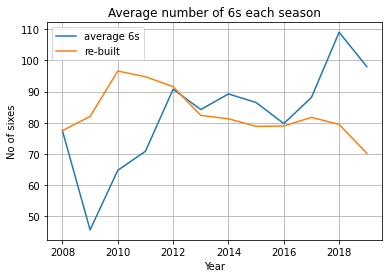
\includegraphics[width=0.5\linewidth]{sixesA}}

\textbf{Predicition:} Total number of sixes = 771\\
\hspace*{75pt} Average number of sixes = 96

\section*{Future Direction}
\begin{enumerate}
\item Including data from Ranji Trophy as it reflects the latest performance of every player, and provides more data for new players or players with insignificant data.
\item To predict the result of each match.
\item To perform online learning, i.e., updating the data as season goes.
\item To also include data of viewership, so as to analyse expected revenue generated from the tournament.
\item To analyse weaknesses for each team.

\end{enumerate}


\end{document}
















